\documentclass[10pt]{article}
\usepackage[utf8]{inputenc}
\usepackage{hyperref}
\usepackage[pdftex]{graphicx}

    
\title{\textbf{Report on Big Data project: \\Analisi delle Aperture nel gioco degli scacchi}}

\author{
	Giovanni Poggi - Mat. 938735}
	
\date{\today}

\begin{document}
\maketitle
\newpage

\tableofcontents

\newpage

\section{Introduzione}

\subsection{Descrizione del Dataset}

Nella realizzazione di questo Progetto si \`e effettuata l'analisi del dataset \textit{Chess Games - 6.2 Million chess games played on LiChess} scaricabile da qui: \url{https://www.kaggle.com/arevel/chess-games?select=chess_games.csv}.\\Il dataset contiene 6,25 milioni di partite di scacchi giocate su \textit{lichess.org} nel Luglio 2016. \`E composto da una sola tabella, in formato csv ed occupa complessivamente 4.1 GB di memoria.

\subsection{Descrizione del file}

La tabella contiene un totale di 15 colonne che descrivono tutti gli elementi caratteristici di una partita di Scacchi.\\Qui di seguito la spiegazione delle colonne presenti:

\begin{enumerate}
    \item \textbf{Evento}: Tipo di gioco; 
    \item \textbf{Bianco}: ID o Nome Utente del giocatore che utilizza le pedine bianche;
    \item \textbf{Nero}: ID o Nome Utente del giocatore che utilizza le pedine nere;
    \item \textbf{Risultato}: Il risultato della partita (1-0 significa che ha vinto il Bianco e 0-1 significa che ha vinto il Nero, altri risultati indicano il pareggio o particolari partite speciali);
    \item \textbf{Data UTC}: Data di inizio partita;
    \item \textbf{Ora UTC}: Ora di inizio partita;
    \item \textbf{WhiteElo}: Valutazione ELO del giocatore Bianco (Sistema di punteggi dei giocatori di scacchi, questo sistema permette la creazione di classifiche a punti autocorrettive nel tempo);
    \item \textbf{BlackElo}: Valutazione ELO del giocatore Nero;
    \item \textbf{WhiteRatingDiff}: Differenza di punti in classifica del bianco dopo la partita;
    \item \textbf{BlackRatingDiff}: Differenza di punti in classifica del nero dopo la partita;
    \item \textbf{ECO}: Apertura in codifica ECO (sistema di classificazione delle aperture);
    \item \textbf{Apertura}: Nome dell'apertura;
    \item \textbf{TimeControl}: Tempo del gioco in secondi;
    \item \textbf{Terminazione}: Motivo della fine del gioco;
    \item \textbf{AN}: Movimenti in formato Movetext;
\end{enumerate}
In particolare, in questo progetto ci si focalizzer\`a principalmente sulle colonne riportanti le Aperture ed il Risultato delle varia Partite effettuate.\\
Qui di seguito un paio di immagini di come si presentano i dati nella tabella:
\begin{figure}[htp]
    \centering
    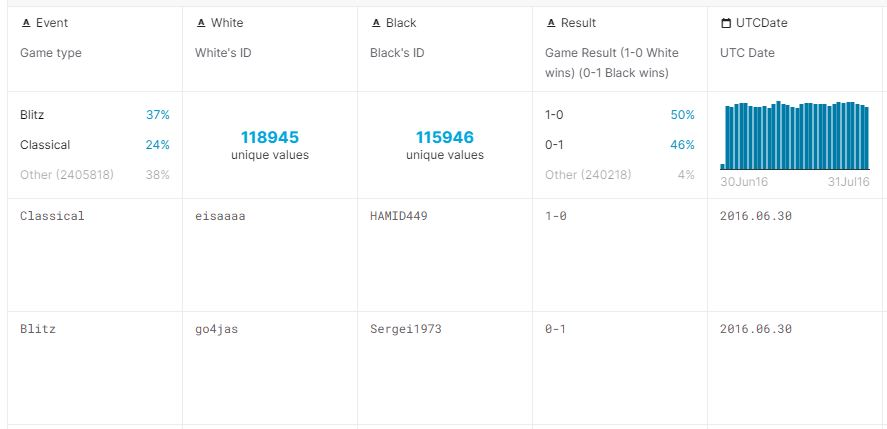
\includegraphics[width=11cm]{images/z1.JPG}
    \caption{First Part of Table CSV}
\end{figure}
\begin{figure}[htp]
    \centering
    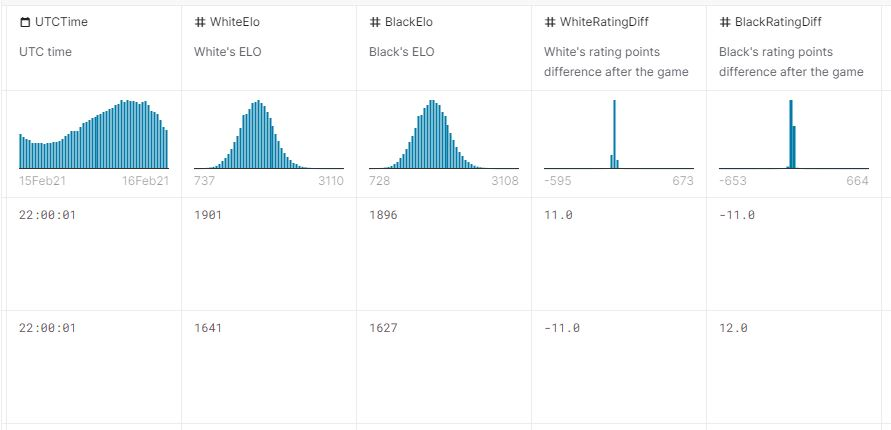
\includegraphics[width=11cm]{images/z2.JPG}
    \caption{Second Part of Table CSV}
\end{figure}
\begin{figure}[htp]
    \centering
    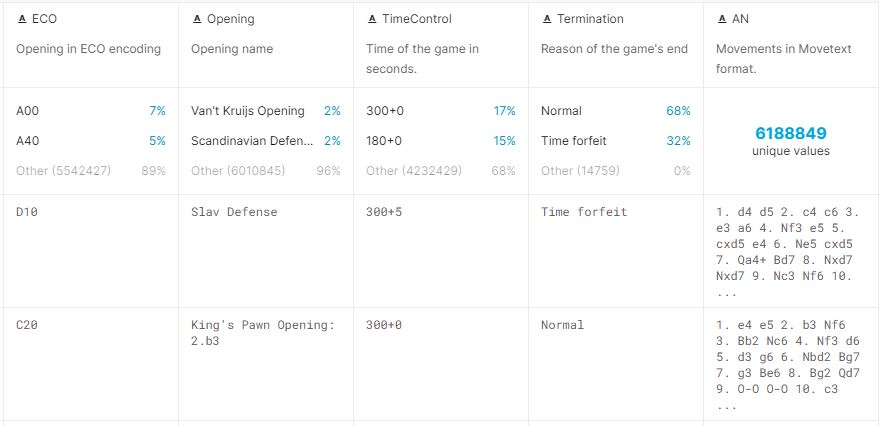
\includegraphics[width=11cm]{images/z3.JPG}
    \caption{Third Part of Table CSV}
\end{figure}

\section{Data Preparation}

Il file utilizzato per questo progetto è stato memorizzato in questo percorso:
\url{hdfs:/user/gpoggi/chessanalysis}.\\Il dataset \`e consistente, non presenta problemi relativi a dati mancanti, non sembrano esserci dati duplicati o di formato errato. Di conseguenza si \`e deciso di non effettuare alcuna operazione di pulizia preliminare dei dati.

\section{Job}

I due job concordati sono stati i seguenti:
\begin{enumerate}
    \item \textit{Date le aperture prese dal dataset, si effettui un calcolo del numero totale di partite in cui sono state utilizzate, quante volte la partita \`e stata vinta, quante persa e quante pareggiata};
    \item \textit{Dati i risultati precedentemente ottenuti, si effettui il calcolo della percentuale di vittorie di tali Aperture e si disponga un ordinamento discendente di tali sulla base della percentuale};
\end{enumerate}
L'implementazione dei due Job \`e stata effettuata con MapReduce e Spark.

\subsection{Implementazione MapReduce}

Il Job \`e stato implementato come lista ordinata di pi\`u Job MapReduce eseguiti in successione. Per una pi\`u corretta comprensione dell'output si \`e pensato di realizzare delle cartelle intermedie create alla fine di ogni Job e memorizzate all'interno dei percorsi \url{hdfs:/user/gpoggi/stageout} e \url{hdfs:/user/gpoggi/outputchess}. La cartella di visualizzazione dell'output finale a fine computazione \`e salvata all'indirizzo \url{hdfs:/user/gpoggi/finaloutput}.\\ Per la realizzazione dell'elaborato si \`e pensato di dividere la consegna in tre Job di MapReduce, descritti qui di seguito.

\begin{figure}[htp]
    \centering
    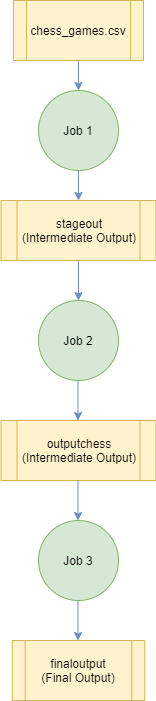
\includegraphics[width=4cm]{images/MapReduce.png}
    \caption{Job Schema}
\end{figure}

\subsubsection{Job 1 - Calcolo totale partite vinte, perse e pareggiate in base all'apertura}

Questo primo Job \`e composto dalle seguenti fasi:

\begin{itemize}
    \item \textbf{Map}: In questa prima operazione si andranno a leggere tutti i dati, riga per riga, dal file di input chess\_games.csv e si manterranno solamente i dati utili ai fini del progetto. L'output di questa Map consiste in coppie chiave-valore del tipo Opening-RisultatoPartita (es. Slav Defense, 1-0);
    \item \textbf{Reduce}: L'operazione di Reduce consiste nel prendere le coppie di valori fornite precedentemente dal Mapper e per ogni Apertura calcolare il numero di partite totali, il numero di partite vinte, il numero delle partite perse ed il numero di partite pareggiate in base allo score assegnato (1-0, 0-1, etc..). In output viene fornito un file di appoggio che possa permettere al secondo Job di eseguire il proprio compito;
\end{itemize}
Il numero di Mapper \`e di 33.\\
Il numero di Reducer scelto \`e di 5.\\
Dopo svariati tentativi si \`e notato che con il numero di default di Reducer (20) il tempo di esecuzione \`e di 1 minuto e 24 secondi circa, di conseguenza si \`e optato per 5 Reducer in quanto il tempo di esecuzione si \`e ridotto a 58 secondi.\\
Si tiene comunque a precisare che questi risultati sono indicativi, in quanto il Cluster poteva essere sovraccarico nel momento dei test. Si \`e comunque tentata diverse volte l'esecuzione del Job e si \`e scelto il risultato migliore.\\
Link YARN: \url{http://isi-vclust0.csr.unibo.it:19888/jobhistory/job/job_1622038346572_0816}

\subsubsection{Job 2 - Calcolo delle percentuali di vittoria ed ordinamento}

Questo secondo Job \`e composto dalle seguenti fasi di elaborazione:

\begin{itemize}
    \item \textbf{Map}: In questa operazione di Map si andranno a leggere i valori salvati dal Job precedemente eseguito e si prenderanno i valori relativi alle colonne delle Vittorie e delle Partite totali andando a calcolare la percentuale di vittorie sul totale delle partite giocate. L'output di questa Map consiste in coppie chiave-valore del tipo Percentuale-StringaPrecedentePresente in modo da effettuare un ordinamento in base alla percentuale grazie al \textit{setSortComparatorClass};
    \item \textbf{Reduce}: L'operazione di Reduce consiste nel ritrasformare i dati precedentemente ottenuti nel formato leggibile e standard su cui si sono eseguiti tutti i precedenti calcoli (Andando quindi a reimpostare come Chiave l'Apertura e come valori tutti i risultati ottenuti precedentemente) ed infine si salveranno i risultati ottenuti nella cartella di \textit{outputchess/};
\end{itemize}
Il numero di Mapper \`e di 5.\\
Il numero di Reducer scelto \`e di 1.\\
Si \`e notato che con il numero di default di Reducer (5) il tempo di esecuzione \`e di 27 secondi, di conseguenza si \`e optato per la scelta di un solo Reducer cos\`i da ottenere un tempo di esecuzione di 20 secondi.\\
Si tiene comunque a precisare che questi risultati sono indicativi, in quanto il Cluster poteva essere sovraccarico nel momento dei test. Si \`e comunque tentata diverse volte l'esecuzione del Job e si \`e scelto il risultato migliore.\\
Link YARN: \url{http://isi-vclust0.csr.unibo.it:19888/jobhistory/job/job_1622038346572_0817}

\subsubsection{Note}

Si precisa che le percentuali del Job 2 possono essere molto variabili o apparire semplicemente troppo alte o basse perch\`e spesso sono aperture utilizzate una sola volta (con vittoria o sconfitta) e di conseguenza la percentuale di successo o fallimento di tale potrebbe risultale del 100\%.

\subsubsection{Job 3 - Calcolo della percentuale di utilizzo dell'apertura}

Questo terzo Job \`e composto dalle seguenti fasi di elaborazione:

\begin{itemize}
    \item \textbf{Map}: In questa operazione di Map si andranno semplicemente a leggere i valori salvati dal Job precedemente eseguito e si effettuer\`a un controllo sulla correttezza del numero di valori in input;
    \item \textbf{Reduce}: L'operazione di Reduce consiste nel calcolare il numero totale di partite giocate e successivamente effettuare il calcolo della percentuale dell'utilizzo di ogni apertura sul totale. Infine verranno ritrasformati i dati precedentemente ottenuti nel formato leggibile e standard su cui si sono eseguiti i precedenti calcoli (Andando quindi a reimpostare come Chiave l'Apertura e come valori tutti i risultati ottenuti precedentemente) e si salveranno i risultati ottenuti nella cartella di \textit{finaloutput/};
\end{itemize}
Il numero di Mapper \`e 1.\\
Il numero di Reducer \`e 1.\\
In quest'ultimo Job non c'erano particolari differenze di esecuzione dato che il numero di Default di Reducer \`e anche quello pi\`u efficiente, con un tempo di esecuzione \`e di 27 secondi.\\
Si tiene comunque a precisare che questi risultati sono indicativi, in quanto il Cluster poteva essere sovraccarico nel momento dei test. Si \`e comunque tentata diverse volte l'esecuzione del Job e si \`e scelto il risultato migliore.\\
Link YARN: \url{http://isi-vclust0.csr.unibo.it:8088/cluster/app/application_1622038346572_0818}

\subsubsection{Note}

Si precisa che le percentuali del Job 3 possono risultare molto spesso troppo basse o nulle perch\`e una determinata apertura viene effettuata molto meno rispetto al totale delle partite giocate. Su grandi numeri, questa percentuale risulter\`a di gran lunga inferiore al 0,001\%.

\subsection{Implementazione Spark}

Nella implementazione degli stessi Job precedenti utilizzando Spark, si \`e utilizzato come output intermedio il percorso \url{hdfs:/user/gpoggi/sparkstageout/} e come output finale il percorso \url{hdfs:/user/gpoggi/sparkoutputchess/} per salvare il file csv finale ottenuto.

\subsubsection{Spark}

Il file di input chess\_games.csv \`e stato caricato in un RDD denominato \textit{chessRdd}. Le operazioni eseguite su questo dataset sono state:
\begin{itemize}
    \item Filtrazione dei dati opportuni dal file di input delle colonne di interesse;
    \item Calcolo del numero totale di partite giocate, partite vinte, partite perse e partite pareggiate e salvataggio su file;
    \item Tramite il file intermedio, calcolo delle percentuali di vittoria e di utilizzo dell'apertura;
    \item Ordinamento per percentuale di vittoria;
\end{itemize}
Per una pi\`u corretta comprensione dei calcoli e dei risultati si \`e pensato di separare le due operazioni di calcolo delle percentuali e salvare i dati intermedi (chess\_games\_output.csv) e finali (chess\_games\_output\_final.csv) in directory separate.\\
Si \`e inoltre provata l'esecuzione dell'implementazione in Spark pi\`u volte, per determinare il miglior numero di \textit{Executor} e \textit{Core per Executor}. Lanciando l'esecuzione con tutte le possibili combinazioni di valori tra i due parametri, si \`e notato che la migliore configurazione per eseguire il programma \`e: \textit{spark2-submit --num-executors 2 --executor-cores 2 --class ChessAnalysisSparkJobs BDE-spark-poggi.jar}. Tramite l'utilizzo di 2 Executors e 2 Core per Executor si riesce ad ottenere un tempo di 42 Secondi circa (Media di tutti i tempi ottenuti). Con tutte le altre configurazioni il tempo impiegato risultava maggiore di tale soglia (Maggiore di 1 Minuto).\\
Si tiene comunque a precisare che questi risultati sono indicativi, in quanto il Cluster poteva essere sovraccarico nel momento dei test. Si \`e comunque tentata diverse volte l'esecuzione del Job e si \`e scelto il risultato migliore.\\
Nella realizzazione del progetto in Spark non \`e stato effettuato caching in quanto gli RDD vengono utilizzati una sola volta.\\
Per una corretta comprensione del lavoro svolto, di seguito il link relativo ai Job in Spark:\\
Link Spark 1: \url{http://isi-vclust0.csr.unibo.it:8088/proxy/application_1622038346572_0827/}\\
Link Spark 2: \url{http://isi-vclust0.csr.unibo.it:18089/history/application_1622038346572_0828}

\begin{figure}[htp]
    \centering
    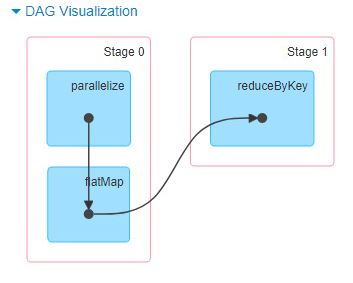
\includegraphics[width=11cm]{images/z4.JPG}
    \caption{DAG Schema Spark 1}
\end{figure}

\begin{figure}[htp]
    \centering
    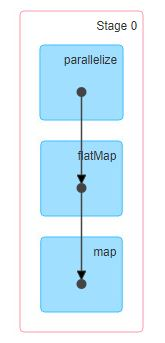
\includegraphics[width=5cm]{images/z5.JPG}
    \caption{DAG Schema Spark 2}
\end{figure}

\subsubsection{Note}

Si precisa che le percentuali dei risultati possono essere molto variabili o apparire semplicemente troppo alte o basse perch\`e spesso sono aperture utilizzate una sola volta (con vittoria o sconfitta) e di conseguenza la percentuale di successo o fallimento di tale potrebbe risultale del 100\%.

\end{document}

%https://vdi.campusfc.unibo.it/portal/webclient/index.html#/desktop
%137.204.72.233:8889 - HUE
%137.204.72.233:7180 - Cloudera Manager